 % ewic.tex for classfile V2.04, 6 July 2011
%per compilare correttamente installare natbib.sty e chicago.bst
\documentclass{ewic}
%\documentclass[cm]{ewic}
\usepackage{graphicx,wrapfig,subfig}
\usepackage{array}
\begin{document}

\runningheads{Ferrari $\bullet$ Mazzanti $\bullet$ Spagnolo}{A model checker solution for the deadlock free the subway}

\conference{Proceedings of  International Workshop on Verification and Evaluation of Computer and Communication Systems 2013}

\title{A model checker solution for the deadlock free the subway[tp]}

\authorone{Alessio Ferrari\\
ISTI-CNR\\
via G. Moruzzi 1 \\56124 Pisa\\
 ITALY\\
fmt.isti.cnr.it\\
\email{alessio.ferrari@isti.cnr.it}}

\authortwo{Franco Mazzanti\\
ISTI-CNR\\
via G. Moruzzi 1\\
56124 Pisa \\
ITALY\\
fmt.isti.cnr.it\\
\email{franco.mazzanti@isti.cnr.it}}

\authorthree{Giorgio O. Spagnolo\\
ISTI-CNR\\
via G. Moruzzi 1 \\
56124 Pisa\\
 ITALY\\
fmt.isti.cnr.it\\
\email{spagnolo@isti.cnr.it}}


\begin{abstract}
This is an abstract.
\end{abstract}

\keywords{Automatic Train Supervisor, CBTC, Deadlock, UMC, Railway, Subway}

\maketitle

\section{Introduction}

This paper describes the ewic.cls class file which can be used to
convert articles produced with other \LaTeXe\ class files into the
correct form for publication by \emph{Electronic Workshops in
Computing}.

The ewic.cls class file preserves much of the standard \LaTeXe\
interface so that any document which has been produced using the
standard \LaTeXe\ article style can easily be converted to work
with the ewic style. However, the width of text and typesize may
vary from that of \emph{article}; therefore \emph{line breaks will
change} and it is possible that computer listings and displayed
mathematics may need resetting.

In the following sections we describe how to lay out your code to
use ewic.cls to reproduce the typographical look required for
online publication. However, this short paper is not a guide to
using \LaTeXe\ and we would refer you to any of the many books
available (see, for example, \cite{Companion,KopkaDaly,Lamport}).

\subsection{eWiC: Information for Authors}
You should also consult \emph{eWiC: Information for Authors} (available
from the BCS website) for important instructions about submission,
style and preparation of your paper.
[studio preliminare]


\section{Background}
%\input{back}
%Esistono sistemi ferroviari di segnalamento e controllo specifici per le metropolitane. I sistemi metropolitani che presentiamo si chiamano Communicated-based Train Control (CBTC).
%Il sistema CBTC è particormente innovativo perchè riceve dai la loro posizione esatta, tramite sistemi wireless. Il sistema è quindi in grado di stabilire delle aeree mobili di sicurezza, al contrario dei vecchi sistemi che utilizzano aree fisse.

% I sistemi CBTC si basano sulle specifiche internazionali
There are railway signalling and train control systems specific to the metro systems. The metropolitan systems that we present are called Communicated-based Train Control (CBTC). CBTC systems are based on international specifications,~\cite{ieee1474} ~\cite{cei2007}.

The conventional metro signalling/control systems the Track circuits are used to detect the presence of trains. Wayside signals are used to ensure safe routes and to provide information to the trains. Therefore, the position of the train is based on the accuracy of the track circuit, and the information provided to the train is limited to the one provided by the wayside signals. These systems are normally referred as \emph{fixed block} systems, since the distance between trains is computed based on fixed-length sections (i.e., the length of a track circuit).

%CBTC overcomes these problems through a continuous wayside-to-train and train-to-wayside data communication. In this way, train position detection is provided by the onboard equipment with a high precision. Furthermore, much more control and status information can be provided to the train. Currently, most of CBTC systems implement this communication using radio transmission~\cite{Kuun2004}. 

The fundamental characteristic of CBTC is to ensure a reduction of the distance between two trains running in the same direction (this distance is normally called \emph{headway}). This is possible thanks to the \emph{moving block} principle: the minimum distance between successive trains is no longer calculated based on fixed sections, as occurs in presence of track circuits, but according to the rear of the preceding train with the addition of a safety distance as a margin. This distance is the limit distance (MA, Movement Authority) that cannot be shortened by a running train. 


%Il sistema CBTC è diviso in diversi sotto-sistemi. I seguenti sottosistemi fanno parte del sistema CBTC : Automatic Train Protecion (ATP), Automatic Train Operation (ATO), Interloking (IXL) e Automatic Train Supervisor (ATS).
The CBTC system is divided into several sub-systems. The following subsystems are part of the CBTC system: Automatic Train Protecion (ATP), Automatic Train Operation (ATO), Interlocking (IXL) and Automatic Train Supervisor (ATS).

%L'Automatic Train Protecion conosce la posizione dei treni sulla linea e la loro velocità.  L'ATP calcola la curva di frenatura per garantire una sufficiente separazione dei treni e controlla che il limite di velocità non sia superato.  Il sistema calcola e assegna al treno l'autorizzazione al movimento. La MA è la distanza limite che un treno non può superare.  L'MA viene usata per garantire la separazione dei treni.
 
The Automatic Train Protecion knows the position of trains on railway and their speed. The ATP calculates the braking curve in order to ensure a sufficient separation of trains and checks that the speed limit is not exceeded. The system calculates and assigns to the train the Movement Authority (MA). %The MA is the limit distance that cannot be shortened by a running train. 
The MA is used to ensure separation of trains.
 
 %Automatic Train Operation è un sistema che permette al treno la guida automatica, sostituendo il macchinista.
 
The Automatic Train Operation is a system that allows the train driving automatically, replacing the driver.
 
 %Interlocking gestisce in sicurezza la linea e gli scambi permettendo o negando l'instradamento dei treni in accordo con le regole di sicurezza ferroviaria.

The Interlocking safely manages the railway and switches allowing or denying routing of trains in accordance with the rules of railway safety.
%L'Automatic Train Supervisor  supervisiona l'intera metropolitana, gestendo il traffico dei treni attraverso i limiti di velocità lo scheduling dei treni ed il loro routing.

The Automatic Train Supervisor supervises the entire subway managing train traffic, through, speed limits, scheduling and routing of trains.

%i sistemi di sicurezza ferroviara impedisco ai treni di scontrarsi, ma non prevengono situazioni di stallo.
%è di fondamentale importanza che i sistemi che gestiscono il traffico ferroviario, non causino delle sistuazioni di stallo o deaadlock.
Railway safety systems prevent to trains of collide, but do not prevent deadlock. Therefore it is of fundamental importance that the systems that manage rail traffic, do not cause situations deadlock.

%Il deadlock ferroviario è una condizione in cui 2 o più treni non possono più continuare la loro missione prevista perchè ogni treno è bloccato da un'altro.
%Una situazione in cui ogni treno è in attesa che un altro treno rilasci una risorsa in una catena circolare.
In railway, the deadlock is a condition in which 2 or more trains cannot  continue their mission expected because each train is blocked by another one.
A situation in which each train is waiting for another train releases a resource in a circular chain,~\cite{Pachl2012}.


%L'ATS quindi dovrà implementare un algoritmo di scheduling e routing che garantisca di non creare situazioni di deadlock. 
%Per capire come impedire che il traffico ferroviario vada in deadlock, introduciamo i seguenti termini specifici.

The ATS will then implement a routing and scheduling algorithm that ensures do not create deadlock. In order to understand how prevent traffic from rail going to deadlock, we introduce the following specific terms.

%timetable is a list of railway journeys arranged according to the time when they arrivals and departures
%La Timetable è una lista di orari e di binari per ogni treno, che indicano la partenza e l'arrivo del treno in ogni stazione.

The Timetable is a list of times and binaries for each train, which indicate the departure time and the arrival time of the train at each station.

%Si presuppone che la timetable sia consistente, cioè che applicanto l'orario i treni non creeranno mai situazioni di deadlock. quindi queste posso crearsi solo in caso di ritardi dei treni.
It is assumed that the timetable is consistent, respecting the time the trains do not ever create deadlock situations. So these can be created only in the case of train delays.

%L'Itinerario è un tratto di linea di una stazione. Quando questo va dall'entrata della stazione al binario di stazionamento si chiama itinerario di ingresso, quando va dal binario di stazionamento all'uscita dalla stazione si chiama itinerario di uscita.

The Itinerary is a section of a railway line. When this goes from the entrance to the station to the tracks of the platform is called ``route of entry'', when it goes from tracks of the platform to the exit station is called ``route of output''.

%La Missione è il servizio affidato ad un treno specifico, che contiene le informazioni riguardanti la stazione di partenza, le fermate da eseguire, in quali binari il treno deve fermasi, quali itinerai deve eseguire per entrare ed uscire dalle stazioni.

The Mission is the service entrusted to a specific train, which contains information about the station of departure and arrival, scheduled stops, in which tracks of the platform must compelled to stop, which routes must perform to enter and exit stations.
 

%In ambito metropolitano, al contrario di quanto accade nella ferrovia tradizione, molto spesso i binari in cui si fermano i treni sono definiti in maniera statica. Questo accade perchè i binari della metropolitana sono pensati prendere....

In metropolitan railway, in contrast to what happens in the railroad tradition, very often binaries where trains stop are defined statically.
 



 
%\begin{enumerate}
%\item Contesto ferroviario: Metropolitate CBTC
%\item Il sistema CBTC
%\item L'ATS il suo compito -> Routing vs TimeTable
%\item definizione di tabella orario 
%\item definizione di missione [statiche siamo in metro]
%\item sicurezza dei treni 
%\item definizione di itinerario 
%\item definizione di deadlock in un sistema ferroviario
%\end{enumerate}



\subsection{Deadlock Pattern definition}

%In figura~\ref{fig:rappresent} è rappresentata di una generica stazione. 
In Figure ~\ref{fig:rappresent} is represented by a generic station.
%In particolare i cerchi con il numero romano rappresentano i binari di stazionamento, mentre gli altri rappresentano punti di ingresso o di uscita alla stazione.
In particular, the circles with the Roman numeral representing the tracks of the platform, while the others circles represent points of entry or exit of the station.
The segment that connects the two circles represents a track of railway line.
 %Il segmento che unisce i due cerchi rappresenta un tratto di linea ferroviaria. 
  %[Due cerchi uniti da un segmento, tutti di colore rosso, rappresentano un itinerario. ]
  [Two circles connected by a segment, all the same color, representing a route.]
 %Il cerchio è colorato quando è presente un treno. Colori diversi indicano treni diversi. Il colore della freccia indica direzione del treno.
The circle is colored when a train is present. Different colors indicates different trains. The color of the arrow indicates the direction of the train.

\begin{figure}[htp]
	\begin{centering}	
	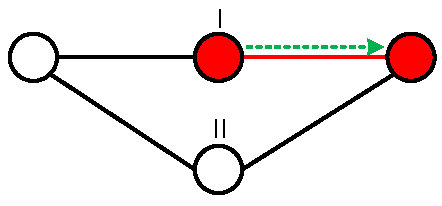
\includegraphics[width=0.3\textwidth, clip]{img/rappresentazione}
	\caption{Generic layout of a station}
	\label{fig:rappresent}
	\end{centering}
\end{figure}

%Dallo studio dei deadlock ferroviari, abbiamo ricavato dei pattern di base. 
%Questi pattern sono usati per riconosce le zone critiche della linea ferroviaria. In queste zone bisogna limitare il numero di treni che è possibile far circolare per evitare di finire in deadlock.
%La composizione di pattern di base permette di identificare tutte le possibili zone in cui è possibile che si crei un deadlock.

From the study of deadlock rail, we have obtained the basic pattern.
These patterns are used to recognize the critical areas of the railway line. In these areas it is necessary to limit the number of trains that it is possible to circulate to avoid ending up in deadlock.
The composition of the basic pattern allows to identify all the possible areas where you may create a deadlock.

%Nella figura~\ref{fig:simpledeadlockpattern} sono disegnati i pattern di base.
In Figure~\ref{fig:simpledeadlockpattern} are represented the basic pattern.

%Nel pattern di base~\ref{fig:lcrossdeadlock} è possibile vedere come entrambi i treni si blocchino a vicenda. Chiameremo questo genere di deadlock:  \emph{``linear deadlock''}. Per eliminare questo deadlock bisogna impedire ad uno dei due treni di entrare in questa sezione critica in direzione opposta. %In questa sezione i treni devo circolare tutti nella stessa direzione.

In the basic pattern~\ref{fig:lcrossdeadlock} is possible to see how both trains block each other. We will call this type of deadlock: \emph{``linear deadlock''}. To eliminate this deadlock must prevent one of the two trains to enter this critical section in the opposite direction. In this section, all trains must move in the same direction.

%Nel pattern ~\ref{fig:circledeadlock} è raffigurata una stazione. Tutti i treni impedisco l'uno l'altro di muoversi. Chiameremo questo genere di deadlock:  \emph{``circle deadlock''}. Per eliminare questo deadlock bisogna impedire che i treni che sono presenti nel ring siamo al massimo N-1. Dove N è la somma dei punti di ingresso o uscita e dei binari di una stazione. Nota: nei singoli segmenti del patter non devono essere presenti treni in direzione contrapposta. i treni  che si trovano al margine del ring e ne stanno uscendo sono ininfluenti

In pattern~\ref{fig:circledeadlock} is represented a ring. All trains block each other. We will call this type of deadlock:  \emph{``circle Deadlock''}. To eliminate this deadlock must prevent that the trains which are present in the ring are at most $N-1$. Where $N$ is the sum of the points of entry or exit and tracks platform of the station. Note: in the individual segments of this patter must not be present trains in the opposite direction. Note2: the trains that are located at the edge of the ring and they are coming out are irrelevant.

\begin{figure}[!htp]
 \centering

 \subfloat[Linear Deadlock Pattern\label{fig:lcrossdeadlock}]{
 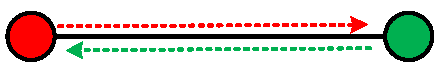
\includegraphics [scale=0.45, clip]{img/deadlinear}
 \label{fig:crossdeadlock}
 }
 \subfloat[Circle Deadlock Pattern\label{fig:lcircledeadlock}]{
 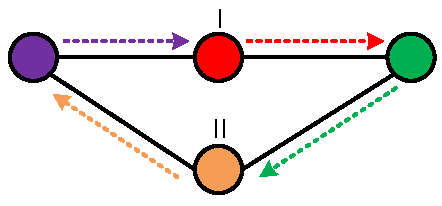
\includegraphics [scale=0.5, clip]{img/circledead}
 \label{fig:circledeadlock}
 }
 

\caption{Simple Deadlock Pattern}
 \label{fig:simpledeadlockpattern}
 \end{figure}


%Tutti gli altri tipi di deadlock sono riconducibili a composizioni di pattern di base.

All other types of deadlocks are referable to compositions of basic pattern.

%\begin{itemize}
%\item definizione della rappresentazione usata
%\item definizione dei deadlock di base:
%\item cross, cicolare o composizione dei precedenti
%\end{itemize}

%\begin{figure}[htp]
%	\begin{centering}	
%	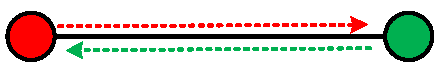
\includegraphics[width=0.43\textwidth, clip]{img/deadlinear}
%	\caption{Linear Deadlock Pattern}
%	\label{fig:linardeadlock}
%	\end{centering}
%\end{figure}

%Nella figura~\ref{fig:compdeadlockpattern} sono rappresentati due pattern composti.

In figure~\ref{fig:compdeadlockpattern} are presented two patterns compounds.

%In figura ~\ref{fig:linecircledeadlock} è disegnato un pattern composto da un circle e una linea. Abbiamo tre zone critiche. Una rappresentata dagli elementi del circle, in questa zona non possono essere presenti più N-1 treni, N=4;  Una rappresentata dagli elementi della linea, in questa zona non possono essere presenti più di un treno nella stessa direzione.
% Una zona critica globale rappresentata da tutto il pattern in cui al suo interno non devo essere presenti treni più di 3 treni, cioè il numero massimo di treni nel pattern circle.

The figure~\ref{fig:linecircledeadlock}  shows a pattern composed of a ``circle pattern'' and a ``linear pattern''. We have three critical areas. The first is represented by the elements of the linear pattern in this area can not be more than one train in the same direction.  The second area is represented by elements of the circle in this area can not be more than $N-1$ trains, with $N=4$; in the main critical area, represented by all patterns,  there must be no more than three trains that is the maximum number of trains in the circle pattern.

\begin{figure}[!htp]
 \centering

 
  \subfloat[Linear and Circle Deadlock Pattern\label{fig:llinecircledeadlock}]{
 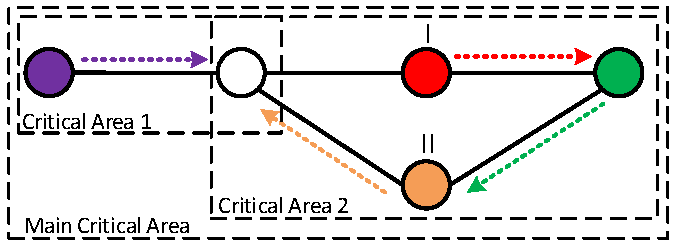
\includegraphics [scale=0.5, clip]{img/linecircledead}
 \label{fig:linecircledeadlock}
 }
 \\
  \subfloat[Double Circle Deadlock Pattern\label{fig:lcircle2deadlock}]{
 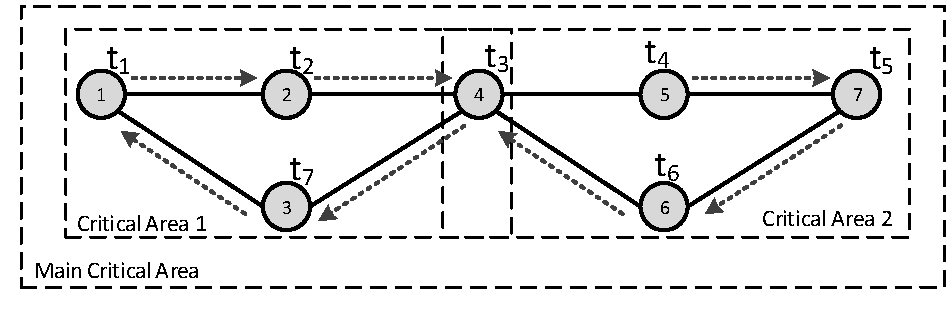
\includegraphics [scale=0.45, clip]{img/circle2dead}
 \label{fig:circle2deadlock}
 }

\caption{Composite Deadlock Pattern}
 \label{fig:compdeadlockpattern}
 \end{figure}

%In figura ~\ref{fig:circle2deadlock}  è disegnato un pattern composto da 2 ring. Abbiamo tre zone critiche. Nelle zone critiche 1 e 2 possono circolare rispettivamente N-1 treni, quindi 3 e 3. Mentre globalmente nei due ring posso circolare ((N-1)+(N-1))-(M-1), dove M è il numero di pattern, quindi massimo 5 treni possono circolare nell'area critica globale.

In Figure ~\ref{fig:circle2deadlock} shows two circle pattern. We have three critical areas. In the critical area one and two can circulate respectively N-1 trains, then three and three. While globally in the two circular ring can circulate $[(N-1) + (N-1)] - (M-1)=5$, where $M$ is the number of patterns, so maximum five trains may run in the main critical area.

\section{Method overview}


%Dati il layout di una metropolitana e la tabella orario dei treni che si vogliono far circolare. Viene definito il modello delle missioni dei singoli treni. Il modello delle missioni unito al modello dello stato della linea formano il modello di scheduling del sistema. 
%Il risultato dell'analisi del model chec ker 

%In questo paragrafo noi descriviamo l'approccio utilizzato per verificare ed eliminare i deadlock in una metropolitana.
%In particolare questa è l'analisi fatta dall'ATS per schedulare i treni in caso di ritardo senza generare deadlock.

In this section we describe the approach used to verify and delete deadlock in a subway.
In particular, this is the analysis performed by the ATS to schedule trains in case of delay without generating deadlocks.

%Il nostro approccio si basa sull'utilizzo iterativo di un model checker per verificare la presenza di deadlock di una metropolitana.

Our approach is based on an iterative model checker to verify the presence of deadlocks of a subway.

\begin{figure}[h!]
	\begin{centering}	
	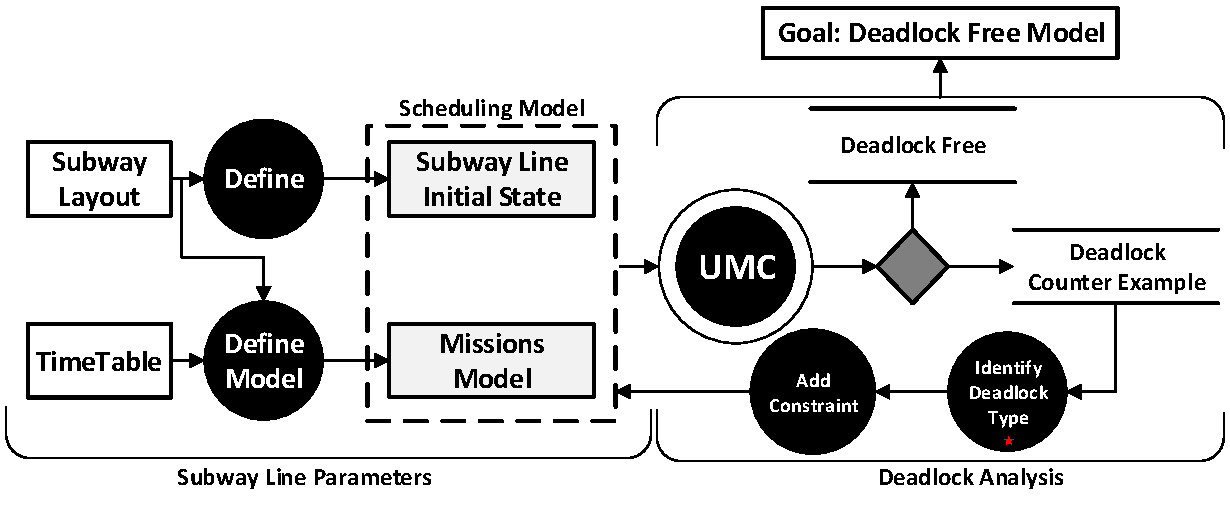
\includegraphics[width=0.45\textwidth, clip]{img/processo}
	\caption{Overview of the approach}
	\label{fig:process}
	\end{centering}
\end{figure}

%La figura~\ref{fig:process} descrive graficamente l'approccio usato.
The figure ~\ref{fig:process} describes the approach used.

%%Nella prima fase, che chiamiamo SLP, vengo preparati i dati per effettuare l'analisi di deadlock della linea.
%I dati di partenza sono  il layout della metropolitana e la tabella orario dei treni che si vogliono far circolare. Questi dati sono usati per definire i modelli delle missioni dei singoli treni. 

The source data are the subway  layout and the metro timetable. Both are used to define models of the missions of individual trains, see figure~\ref{fig:lmissionm}.


%Invece il layout della metropolitana viene usato anche per definire lo stato iniziale della linea. Cosi è possibile bloccare alcuni tratti di metropolitana perchè impegnati ad esempio da lavori di manutenzione.

Whereas the layout of the subway is also used to define the initial state of the line, see figure~\ref{fig:lstateline}. So you can lock some parts of the subway because it involved such as maintenance or insert the initial position of train.

%I modelli di missione e lo stato iniziale della metropolitana costituiscono il modello di scheduling della metropolitana.

The models of the mission and the model initial state of the subway they represent the model of scheduling of the subway, see figure~\ref{fig:SchedulingModel}.

%Il modello di scheduling viene analizzato tramite il model checker UMC[inserire riferimento]
The scheduling model is analyzed using the model checker UMC [insert reference]
%UMC permette di specificare come un insime di statecharts UML e di verificare proprità relative all'evoluzione del sistema. 
UMC allows to specify a system as a set of UML Statecharts and verify properties related to the evolution of the system.

%Se risultato del modelchecker è controesempio di deadlock. Si identificano i pattern di deadlock e si inserisco delle nuove regole nelle aree scritiche identificate. Altrimenti potremo affermare che il modello è libero di deadlock.

If the result of the model checker is deadlock counter example we identify patterns of deadlocks and insert the new contraints in the critical areas identified, see section~\ref{sec:deadlockpatterndefinition}. Otherwise, we can conclude that the model is free of deadlocks. 
%Quindi tutti i treni sono ingrado di arrivare a destinazione senza generare deadlock.
So all the trains, present into timetable, are able to arrive at your destination without generating deadlock.

\section{DeadLock Analysis}

\begin{figure}[htp]
	\begin{centering}	
	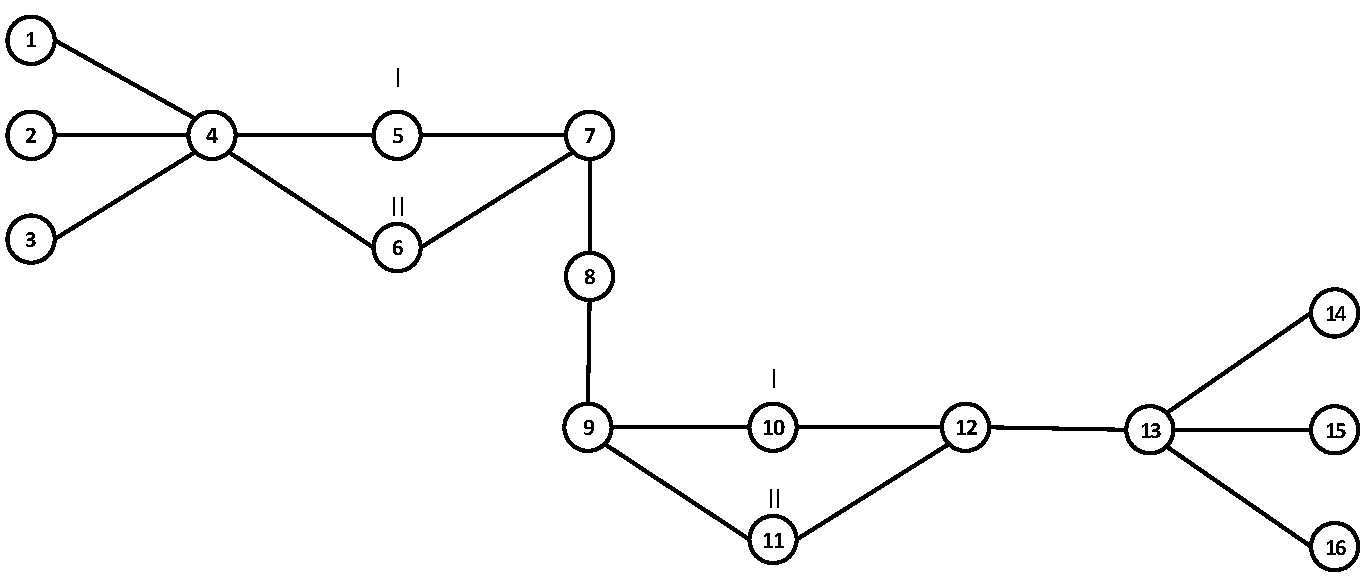
\includegraphics[width=0.45\textwidth, clip]{img/esempio}
	\caption{Layout of a simple subway}
	\label{fig:example}
	\end{centering}
\end{figure}


\begin{enumerate}
\item introduzione del caso concreto
\item presentazione layout dell'esempio
\item presentazione di una sez di tab orario
\item presentazione stato linea
\item definizione del modello di missione
\item contro esempio di deadlock generato da umc
\item riconoscimento del tipo di deadlock
\item aggiunta di una nuova regola al modello
\item \ldots ripeto dal passo 6 finch\'{e}
\item GOal: tabella orario libera da deadlock
\end{enumerate}
%\input{example}

\section{Related works}
%\input{releted}
\section{Conclusion}
%\input{conclusion}



\pagebreak
\subsection{Notes}
\begin{enumerate}
\item Please separate multiple author surnames by a `\verb+$\bullet$+' within the
\verb+\runningheads{}{}+ command.

\item The class file is set up to handle up to six authors, i.e., \verb+\authorone{}...\authorsix{}+.

\item Note that the required reference style is Harvard. ewic.cls
uses `natbib.sty' to achieve the desired output so you will need
to choose a natbib compatible .bst that gives Harvard style
output. `chicago.bst' would be a good choice.

\item Try to balance the columns on the final page when your paper is submitted.
\end{enumerate}

That really is all you should need to know to prepare your paper
using ewic.cls.\citep{Mills2003}

You do, of course, have the option to call in any of your
favourite packages for setting maths, graphics, computer listings,
etc.

\textbf{Acknowledgments. }
This work was partially supported by the PAR FAS 2007-2013 (TRACE-IT) project.

%\begin{thebibliography}{9}
%
%\bibitem[Kopka and Daly(2004)]{KopkaDaly}
%Kopka, H. and Daly, P.W.  (2004) \textit{A Guide to \LaTeXe:
%Document Preparation for Beginners and Advanced Users} (4th~edn).
%Addison-Wesley.
%
%\bibitem[Lamport(1994)]{Lamport}
%Lamport L. (1994) \textit{\LaTeX: A Document Preparation System}
%(2nd~edn). Addison-Wesley.
%
%\bibitem[Mittelbach and Goossens(2004)]{Companion}
%Mittelbach, F. and Goossens, M., (2004) \textit{The \LaTeX\
%Companion} (2nd~edn). Addison-Wesley.
%
%\end{thebibliography}

\bibliographystyle{chicago}
\bibliography{bibliography}


\end{document}
